\documentclass[11pt]{article}
\usepackage[margin=0.85in]{geometry}
\usepackage{amsmath,amssymb,booktabs,array,xcolor,hyperref,tikz}
\usetikzlibrary{arrows.meta,positioning}
\hypersetup{colorlinks=true,urlcolor=teal,linkcolor=teal}
\setlength{\parindent}{0pt}\setlength{\parskip}{6pt}
\newcommand{\idea}[1]{\textbf{Main idea.} #1}
\begin{document}
\begin{center}{\LARGE Understanding SIR models, one flow at a time}\\[7pt]
{\large Beginner mathematical and statistical reading notes}\\
Prepared for Md. Ikramul Haq Khan --- MS thesis literature review\\
Version 1.0 $\mid$ October 25, 2026
\end{center}
\textbf{Reading context.} Companion to Fudolig and Howard (2020), Figure 1 and the ``Before emergence'' discussion, especially the passage on birth/death, vaccination, transmission and removal coefficients. This note also consolidates the earlier compartment explanation in this conversation. These are learning notes, not an approved thesis specification or a claim of new results.
\section{People, groups, and time}
\idea{A compartment is a group of people with the same modeled disease status.}
\begin{center}\begin{tabular}{ll}\toprule
Symbol & Meaning at time $t$\\\midrule
$S(t)$ & Susceptible: can catch the original strain\\
$I_1(t)$ & Infectious with strain 1 (the original strain)\\
$R(t)$ & Recovered and protected against strain 1\\
$V(t)$ & Vaccinated/protected against strain 1\\
$N$ & Total population: $S+I_1+R+V$\\\bottomrule
\end{tabular}\end{center}
The subscript 1 labels the strain; it does not mean one infected person. The paper also includes naturally immune people in $V$. Here we explain the vaccination mechanism shown in its figure.
\begin{center}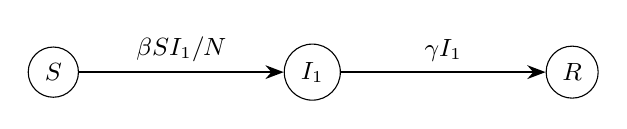
\begin{tikzpicture}[>=Stealth,node distance=2.6cm,every node/.style={font=\small}]
\node[draw,circle] (s) {$S$};\node[draw,circle,right=of s] (i) {$I_1$};\node[draw,circle,right=of i] (r) {$R$};
\draw[->,thick] (s)--node[above] {$\beta SI_1/N$}(i);
\draw[->,thick] (i)--node[above] {$\gamma I_1$}(r);
\end{tikzpicture}\end{center}
This simplified path shows infection and recovery. Births, vaccination and deaths are added below. Each arrow label is a \emph{flow rate}, measured in people per unit of time.
\section{A dictionary of the parameters}
\begin{center}\begin{tabular}{p{0.11\linewidth}p{0.56\linewidth}p{0.21\linewidth}}\toprule
Symbol & Interpretation & Units\\\midrule
$\mu$ & Per-person natural death rate; also the birth coefficient & time$^{-1}$\\
$p$ & Fraction of newborns vaccinated, $0\leq p\leq1$ & no units\\
$\beta$ & Transmission coefficient & time$^{-1}$\\
$\gamma$ & Recovery/removal coefficient from infection & time$^{-1}$\\\bottomrule
\end{tabular}\end{center}
\textbf{Distinguish state from parameter:} $I_1(t)$ changes along a trajectory; a fixed $\gamma$ describes the rule governing recovery. A coefficient is not itself the total flow. Although the paper calls $p$ a vaccination rate, it functions here as a proportion of births.
\newpage
\section{Why births and deaths use $\mu$}
\idea{Multiply a per-person rate by a group size to obtain a total flow.}
Births enter at rate $\mu N$. Of these, fraction $p$ enter $V$ and fraction $1-p$ enter $S$:
\[
\text{births into }S=(1-p)\mu N,\qquad
\text{births into }V=p\mu N.
\]
Natural deaths leave each compartment at rates $\mu S$, $\mu I_1$, $\mu R$ and $\mu V$. For example, $\mu S$ has units $(\text{day}^{-1})(\text{people})=\text{people/day}$ if days are the time unit.
If total births are 10 per unit time and $p=0.7$, 7 enter $V$ and 3 enter $S$. These are illustrative numbers, not estimates from the paper.
\textbf{Model assumption:} newborns receive vaccination at entry. There is no adult $S\to V$ transition in Figure 1. Vaccination fully protects against strain 1, with no waning in this baseline.
\section{Why infection has flow $\beta SI_1/N$}
\idea{More infectious people increase exposure; more susceptible people create more opportunities for new infection.}
\[
\lambda(t)=\beta\frac{I_1(t)}{N},\qquad
\text{total infection flow}=\lambda(t)S(t).
\]
Here $I_1/N$ is the infectious fraction. The quantity $\lambda$ is the infection \emph{hazard}: the instantaneous infection rate per susceptible person. Under homogeneous mixing, contacts encounter infectious people according to their population fraction. One interpretation is $\beta=cq$, with $c$ contacts per person per unit time and $q$ transmission probability per relevant contact.
\textbf{Standard incidence:} with $c$ fixed, doubling population size at the same infectious fraction leaves each susceptible person's hazard unchanged. Total infections double if $S$ doubles. This differs from a density-dependent term $\widetilde\beta SI_1$, whose coefficient has different units.
\textbf{Worked example.} Let $N=1000$, $S=800$, $I_1=50$, and $\beta=0.4$ per day. Then
\[
\lambda=0.4\frac{50}{1000}=0.02\text{ per day},\qquad
\lambda S=0.02(800)=16\text{ people/day}.
\]
This is the instantaneous flow, not a guarantee of exactly 16 infections tomorrow. If $S=0$ or $I_1=0$, the infection flow is zero.
\section{Why recovery has flow $\gamma I_1$}
Each infectious person has recovery hazard $\gamma$, so the total recovery flow is $\gamma I_1$. If $\gamma=0.2$ per day and $I_1=50$, it is 10 people/day.
With constant recovery hazard and no competing exit, infectious duration is exponential with mean $1/\gamma=5$ days in the corresponding Markov interpretation. With natural death also possible, time until either recovery or death has mean $1/(\gamma+\mu)$. The ODE itself tracks continuous group totals, not individual waiting times.
\newpage
\section{Translate arrows into differential equations}
\idea{For every group: rate of change equals total inflow minus total outflow.}
For a general compartment $C(t)$,
\[
\frac{dC}{dt}=\text{inflow}-\text{outflow}.
\]
The derivative $dC/dt$ describes the slope right now. For a small interval $h$,
$C(t+h)\approx C(t)+h\,dC/dt$. The approximation gets better as $h$ shrinks when the solution is smooth.
Reading all arrows gives
\begin{align*}
\frac{dS}{dt}&=(1-p)\mu N-\frac{\beta SI_1}{N}-\mu S,\\
\frac{dI_1}{dt}&=\frac{\beta SI_1}{N}-\gamma I_1-\mu I_1,\\
\frac{dR}{dt}&=\gamma I_1-\mu R,\\
\frac{dV}{dt}&=p\mu N-\mu V.
\end{align*}
\textbf{Read the infectious equation aloud:} the infectious group gains new infections and loses recoveries and natural deaths. With the previous example and $\mu=0.001$ per day, its net change is $16-10-0.05=5.95$ people/day. Fractional values are legitimate in this continuous approximation.
\textbf{Conservation check.} Adding the four equations cancels internal transfers:
\[
\frac{dN}{dt}=\mu N-\mu(S+I_1+R+V)=0.
\]
Thus total population stays fixed because births balance deaths. Individual compartments can still change. Here a closed population means no migration; births and deaths are explicitly allowed.
\section{When does infection increase?}
Factoring the infectious equation gives
\[
\frac{dI_1}{dt}=I_1\left(\beta\frac{S}{N}-(\gamma+\mu)\right).
\]
For $I_1>0$, infection increases when $\beta S/N>\gamma+\mu$. Intuitively, each infectious person generates infections faster than people leave the infectious group.
Define the basic reproduction number for this baseline by
\[
\mathcal R_0=\frac{\beta}{\gamma+\mu}.
\]
It combines transmission with mean time before recovery/death in a fully susceptible population. The current effective value is $\mathcal R_{\rm eff}(t)=\mathcal R_0 S(t)/N$. At the disease-free equilibrium, $S/N=1-p$, so $\mathcal R_v=\mathcal R_0(1-p)$. The threshold concerns growth near that state; it does not guarantee persistence in every random simulation.
\newpage
\section{Statistical meaning: rates are not probabilities}
\idea{A rate describes how quickly events occur; a probability describes the chance of an event over an interval.}
For a constant isolated hazard $a$, the probability of its event within time $h$ is $1-e^{-ah}$, approximately $ah$ for small $h$. If $\lambda=0.02$ per day and exposure stays constant with no competing exits, the one-day infection probability is $1-e^{-0.02}\approx0.0198$. A hazard need not be below 1; a probability must be.
\textbf{A possible stochastic extension.} At the current state, an infection event changes $(S,I_1,R,V)$ by $(-1,+1,0,0)$, with event rate $a_{\rm inf}=\beta SI_1/N$. A recovery changes it by $(0,-1,+1,0)$, with rate $a_{\rm rec}=\gamma I_1$. For a sufficiently small $h$, the probability of one specified event type is $a_k h+o(h)$. This is a local approximation, not an unrestricted time-step formula.
These random events generate different trajectories even with identical parameters. Nonlinear mean dynamics generally do not close exactly: $E[SI_1]\ne E[S]E[I_1]$ in general. Therefore the deterministic curve need not equal the exact stochastic mean.
\textbf{Population-size caution.} Independent random birth/death events allow the total population to fluctuate even though their deterministic drifts balance. An exactly fixed-$N$ stochastic model requires a compatible replacement mechanism and adviser confirmation. This note does not choose the thesis event mechanism.
\section{Connect to infection curves and distribution fitting}
Prevalence $I_1(t)$ counts people currently infectious. Incidence flow $j(t)=\beta S(t)I_1(t)/N$ counts new infections per time. They have different areas:
\[
A_T=\int_0^T I_1(t)\,dt\quad\text{(infectious person-time)},\qquad
C_T=\int_0^T j(t)\,dt\quad\text{(new infections)}.
\]
For time in days, 10 infectious people for 3 days contribute 30 person-days. This does not identify the number of distinct infected people. Finite horizon $T$ must be specified; persistent positive prevalence makes infinite-horizon prevalence area diverge.
In repeated stochastic runs, $A_T^{(1)},\ldots,A_T^{(B)}$ form a sample of epidemic burdens. A distribution fit describes their variation across runs. Fitting a curve over time is a separate task; successive time points are not independent repeated epidemics. Confirm the target, initial state, horizon and parameter settings with the adviser before fitting.
\section{Reference and learning checks}
Fudolig, M., and Howard, R. (2020). The local stability of a modified multi-strain SIR model for emerging viral strains. \emph{PLOS ONE}, 15(12), e0243408. \url{https://doi.org/10.1371/journal.pone.0243408}. Baseline definitions follow this source; worked numbers and statistical explanations are instructional additions.

\textbf{Check your understanding:} Why does infection appear with opposite signs in $S$ and $I_1$? Why is $p$ unitless? Why does constant $N$ not imply constant $I_1$? What changes if the curve is incidence rather than prevalence? Explain each in words before manipulating equations.
\newpage
\section{Cited papers relevant to this passage}
The bracketed numbers below follow Fudolig and Howard (2020), not a new bibliography numbering scheme. These entries are selected readings; a citation does not mean full-text critical appraisal has been completed.

\subsection*{Reference 66: transmission assumptions (secondary priority)}
Han, L., Ma, Z., and Hethcote, H. (2001). Four predator prey models with infectious diseases. \emph{Mathematical and Computer Modelling}, 34(7--8), 849--858.
\url{https://doi.org/10.1016/S0895-7177(01)00104-2}.

\textbf{Why it appears here.} The source paper cites this work when introducing its infection-transmission assumption. Its setting combines predator-prey dynamics and infection, rather than the present human epidemic model.

\textbf{Thesis use.} Consult for background on incidence choices if needed. It is lower priority than a direct SIR introduction. Do not add predator-prey dynamics to the thesis because this reference appears in the source. Identification and broad relevance are based on the source bibliography and publisher abstract/record; full text was not appraised.

\subsection*{Reference 67: SIR, vaccination and stability (more direct)}
Zaman, G., Kang, Y. H., and Jung, I. H. (2008). Stability analysis and optimal vaccination of an SIR epidemic model. \emph{BioSystems}, 93(3), 240--249.
\url{https://doi.org/10.1016/j.biosystems.2008.05.004}.
PubMed: \url{https://pubmed.ncbi.nlm.nih.gov/18584947/}.

\textbf{What it studies.} The abstract describes an SIR model, equilibrium/stability analysis, and a vaccination control problem, with numerical simulation.

\textbf{Thesis use.} A more direct background reading for understanding SIR equations, vaccination and equilibrium concepts. Optimal control is an additional topic, not a confirmed thesis aim. Relevance is based on the abstract and how Fudolig and Howard cite it; detailed assumptions must be checked in the full paper before transferring formulas.

\subsection*{How to place these in the literature review}
Use both as mathematical-modeling background. Neither has been established here as a distribution-fitting study for infection curves or AUC. A separate targeted review is needed before claiming a gap in that statistical contribution.

For Zotero, use each DOI in Add Item by Identifier. Keep the source paper's reference numbers in notes only; the final thesis bibliography will have its own numbering.

\end{document}
